\documentclass{beamer}
\usepackage{kotex}
\usetheme{metropolis} % Metropolis theme is modern and minimalistic
%\usetheme{Madrid} % Fee6l free to change the theme
%\usetheme{Berkeley}

% Define custom colors (choose colors that suit your style)
\definecolor{PrimaryColor}{RGB}{36, 123, 160}
\definecolor{SecondaryColor}{RGB}{112, 193, 179}

\setbeamercolor{palette primary}{bg=PrimaryColor,fg=white}
\setbeamercolor{palette secondary}{bg=SecondaryColor,fg=white}

% Add any packages you need here
\usepackage{graphicx}
\usepackage{booktabs}
\usepackage{tikz}
\usepackage{hyperref}

\title[Short Title]{PUBAO - Over the Long Long}
\subtitle{Project: P.A.N.D.A.'s Unbounded Big Arithmetic Operations}
\author{Team: Programmers Aspiring to Navigate Digital Arithmetic (P.A.N.D.A)}
\institute{국민대학교 과학기술대학 정보보안암호수학과}
\date{\today}

\begin{document}
	
	\begin{frame}
		\titlepage
	\end{frame}
	
	\begin{frame}{목차}
		\tableofcontents
	\end{frame}

\section{I. 개발자들아, 나와라!}

\begin{frame}{개발진 소개}
	% Use two columns: one for photos and one for text
	\begin{columns}
		\column{0.4\textwidth}
%		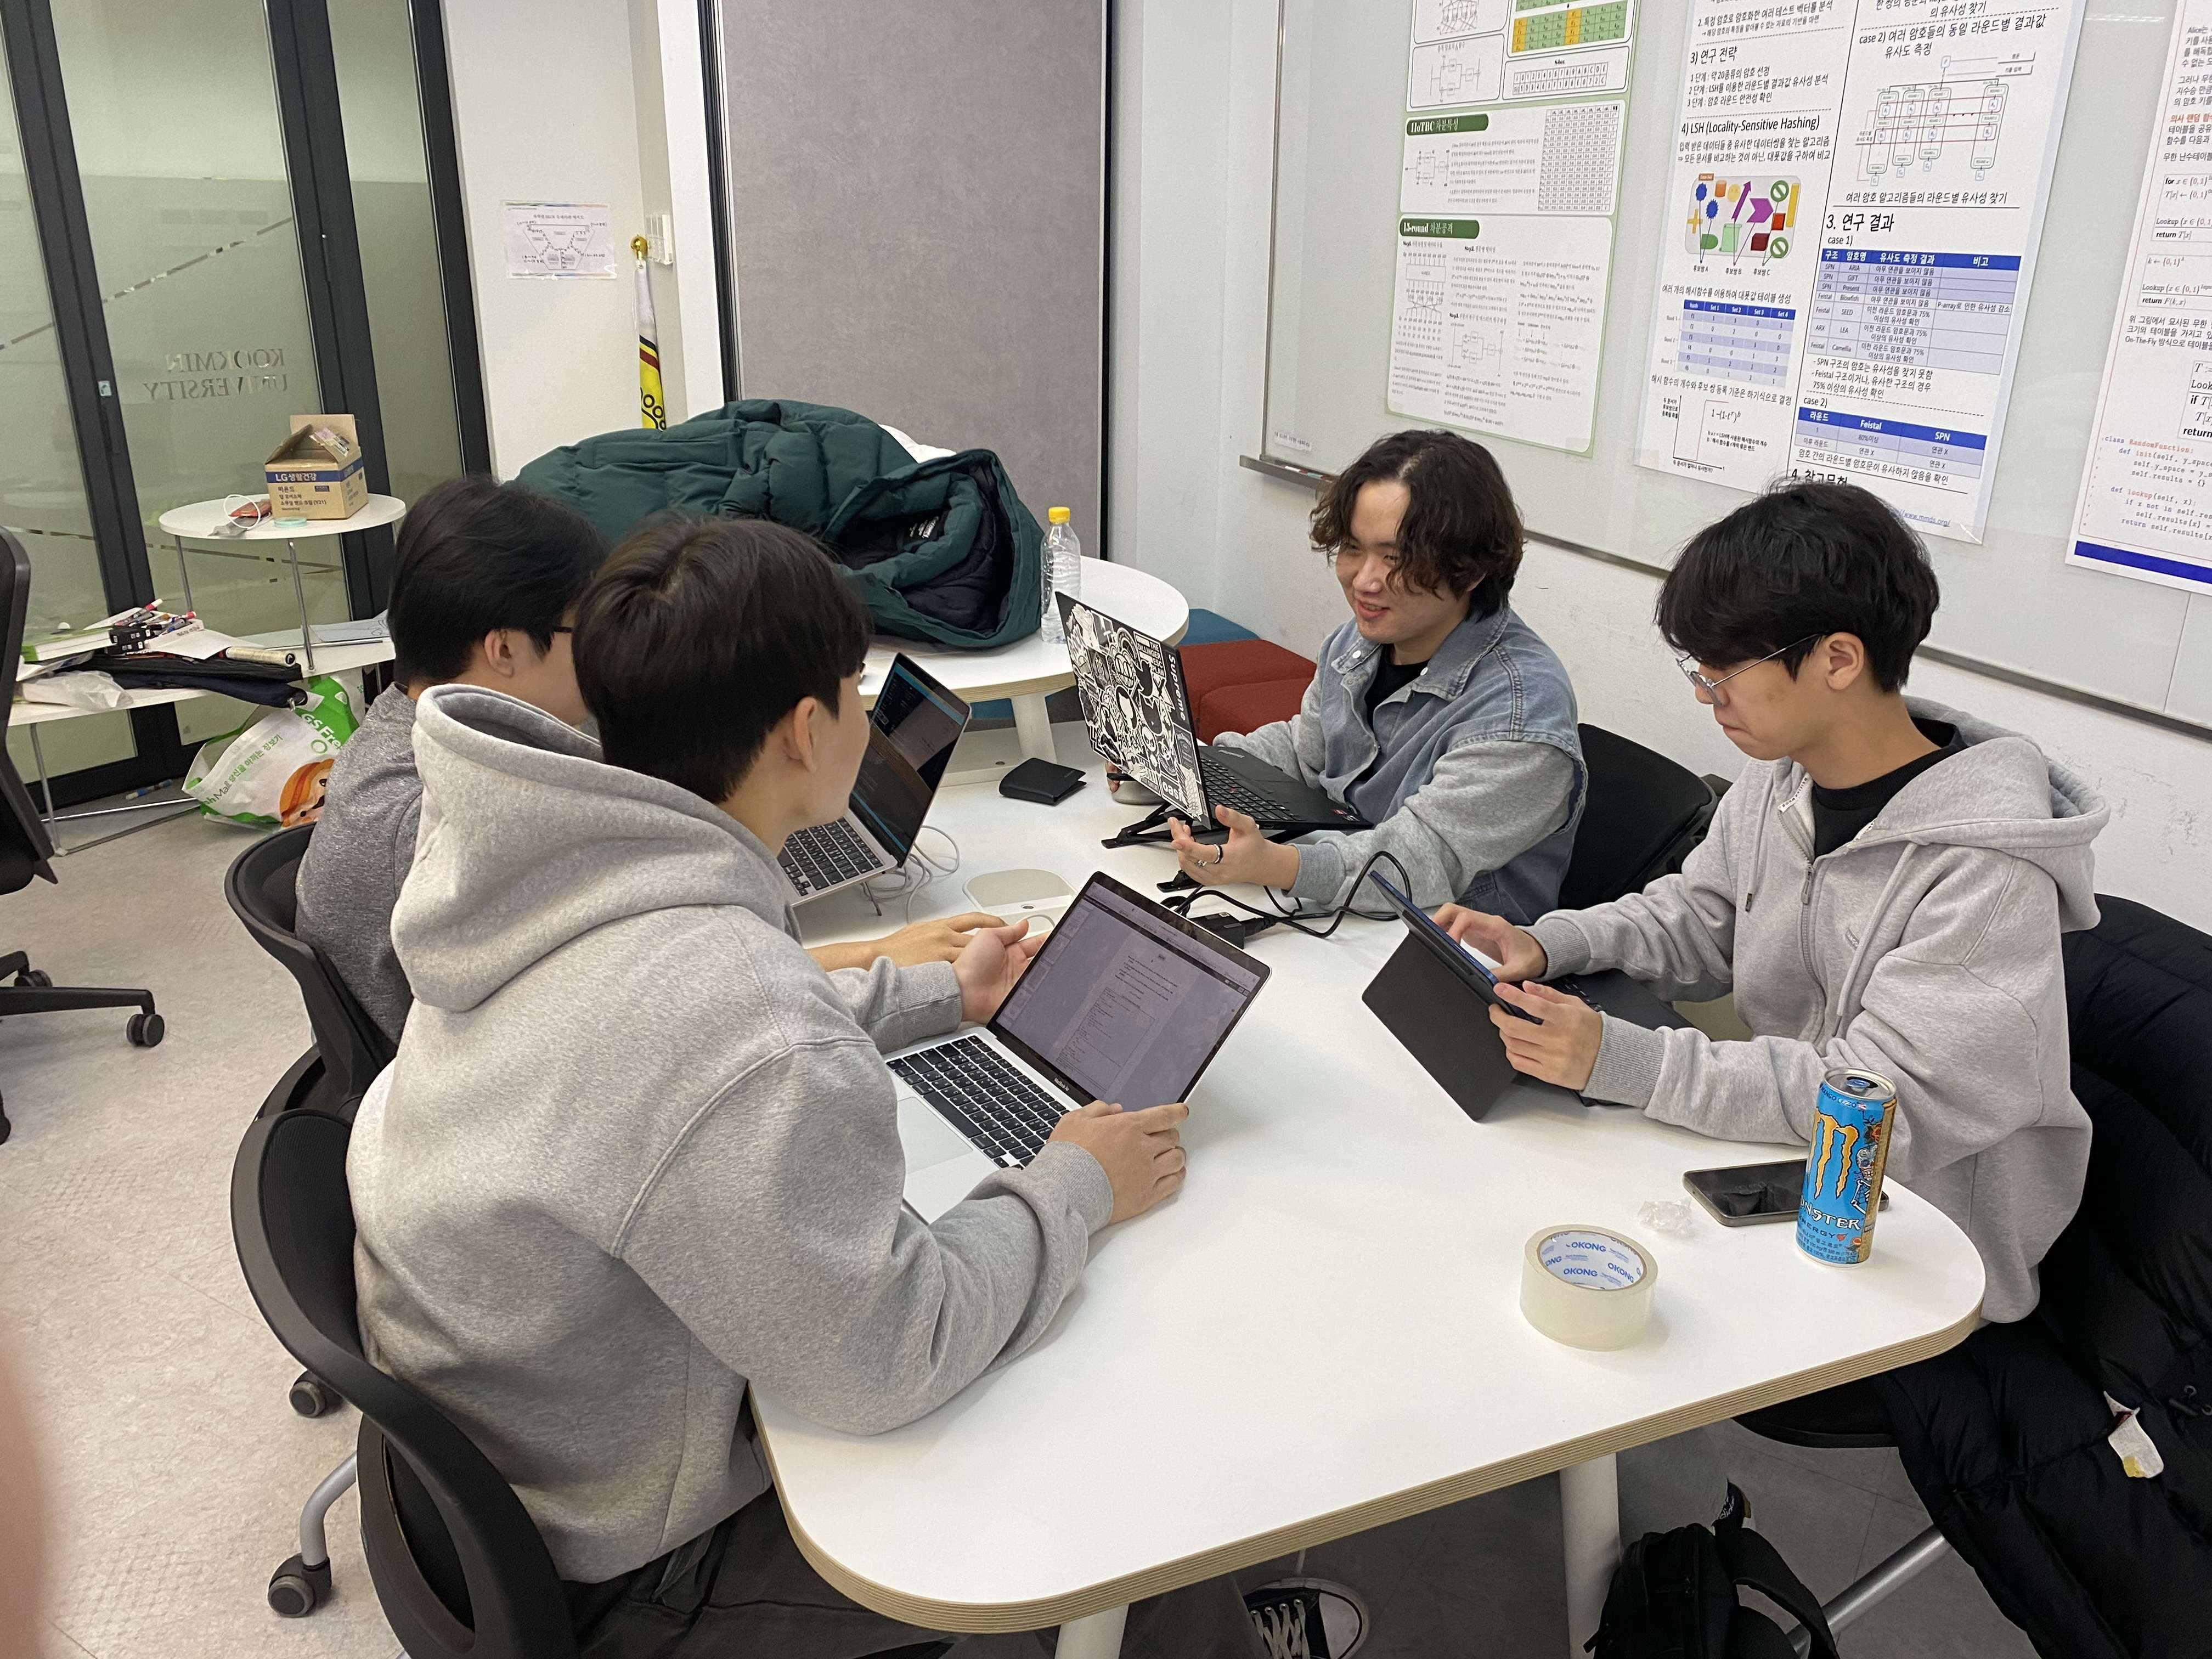
\includegraphics[width=\textwidth]{team_photo.jpg}
		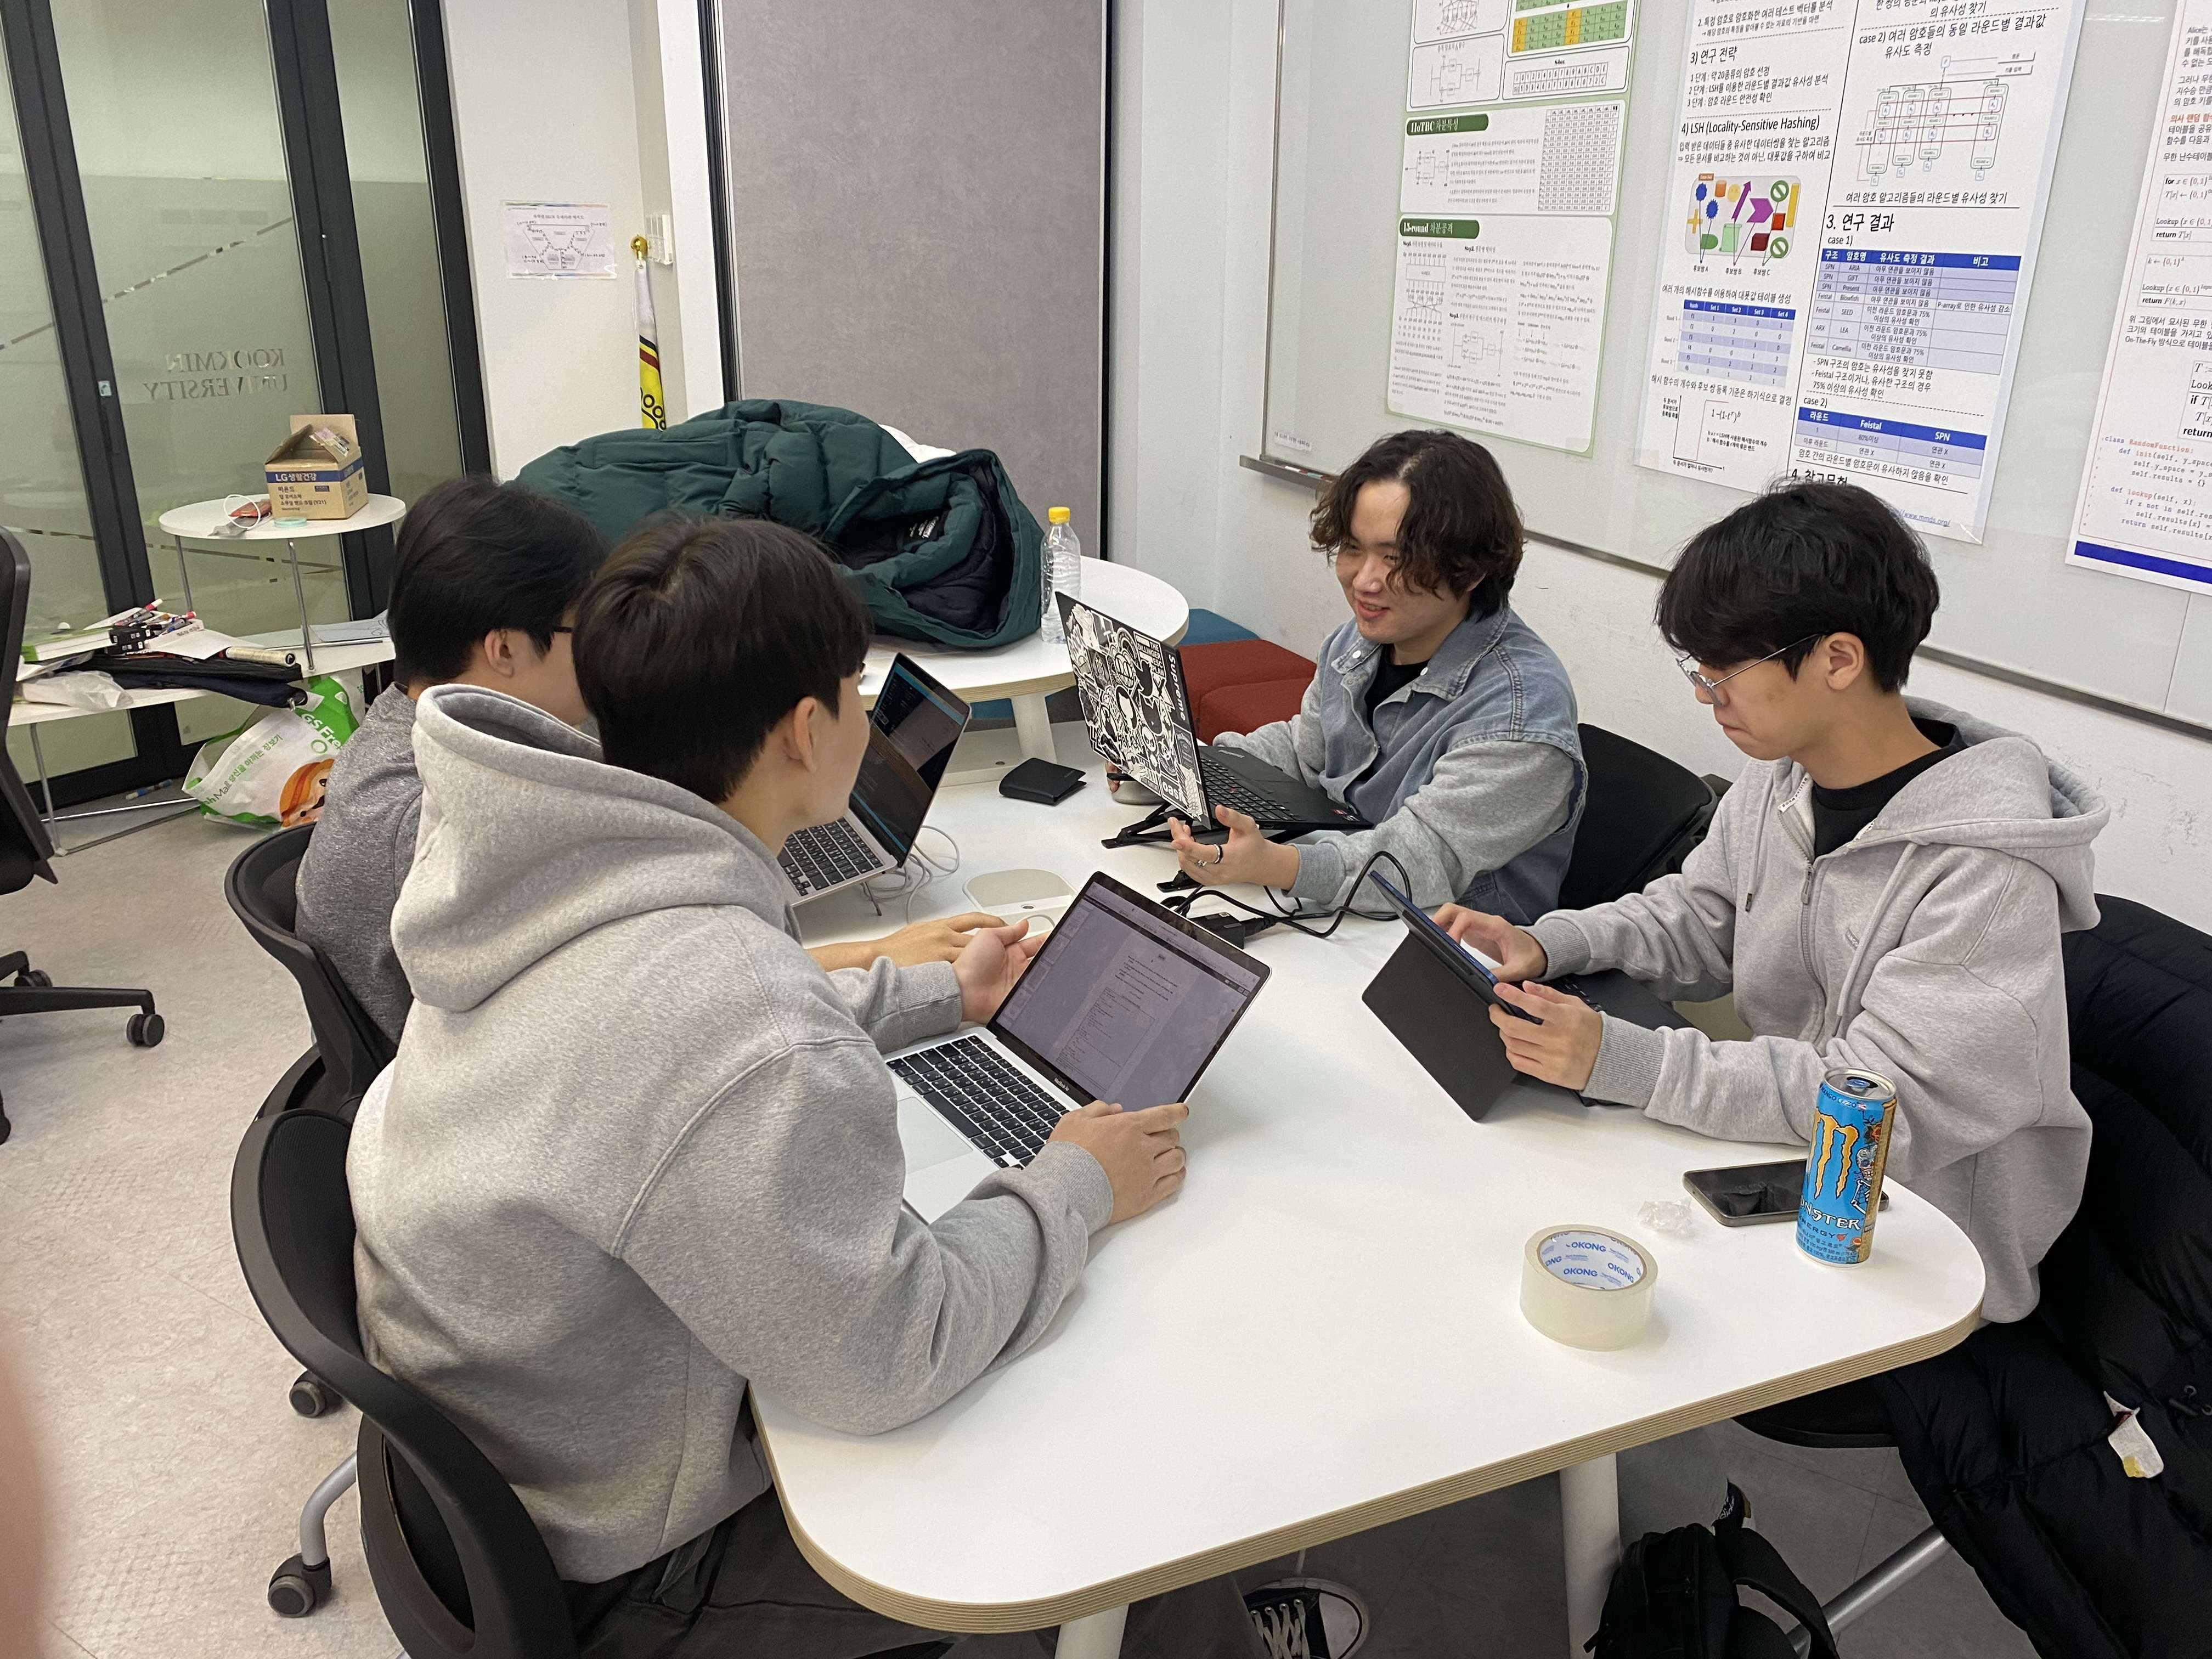
\includegraphics[scale=.035]{team_photo.jpg}
		\column{0.5\textwidth}
		% List your team members and roles here
		\begin{itemize}
			\item 지용현(20192250, Leader)
			\item 문예찬(20192230, Builder)
			\item 김예찬(20192220, Validator)
			\item 유근오(20232093, Intern)
			% Add more members as needed
		\end{itemize}
	\end{columns}
\end{frame}

\begin{frame}{I.1 팀원 소개}
	\begin{columns}[T,onlytextwidth]
		\column{0.5\textwidth}
		\centering
		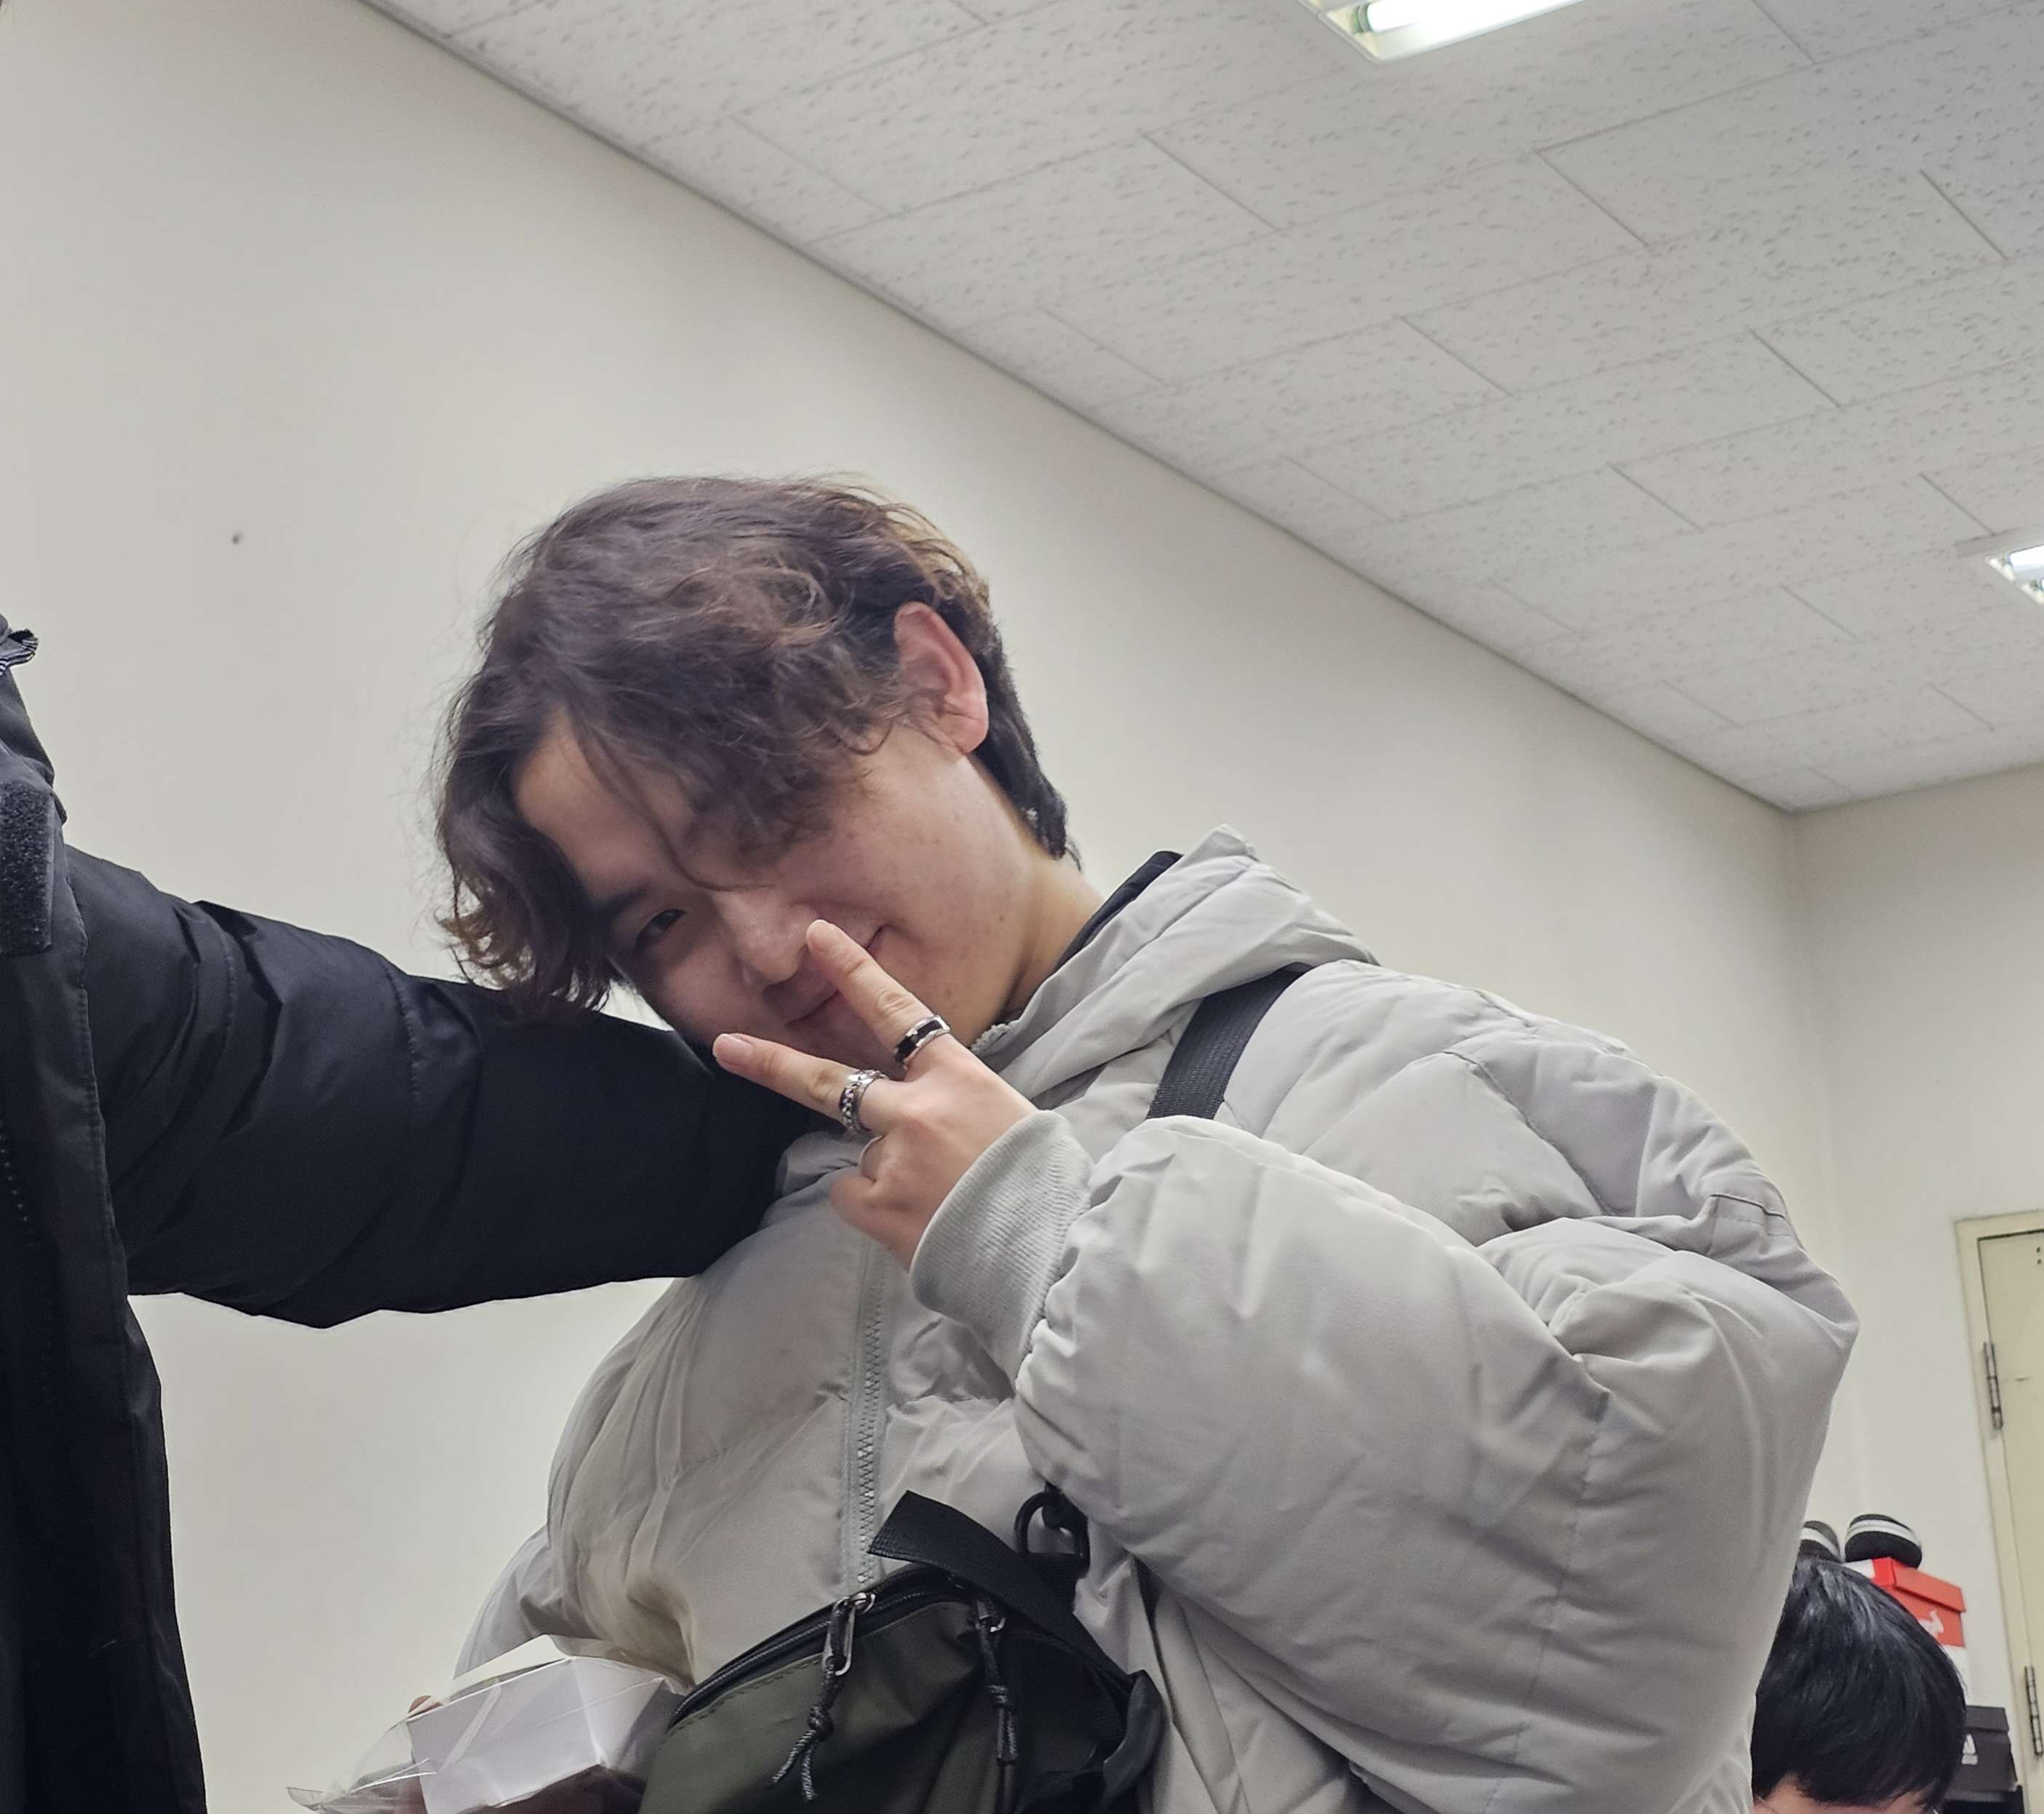
\includegraphics[width=.5\linewidth,height=.35\textheight]{ji.jpg}\\
		\textbf{지용현 (Leader)}\\
		\textit{``위대한 리더''}\\
		\begin{flushleft}\footnotesize
			특징: 전국민초사랑연맹 임원\\
			한마디: \textbf{버그가 아니라 이스터에그다}
		\end{flushleft}
		
		\column{0.5\textwidth}
		\centering
		
\includegraphics[width=.5\linewidth,height=.35\textheight]{PANDA_logo.png}\\
		\textbf{유근오 (Intern)}\\
		\textit{``꿈꾸는 샛별''}\\
		\begin{flushleft}\footnotesize
			특징: -\\
			한마디: -
		\end{flushleft}
	\end{columns}
\end{frame}
\begin{frame}{I.2 팀원 소개}
	\begin{columns}[T,onlytextwidth]	
		\column{0.48\textwidth}
		\centering
		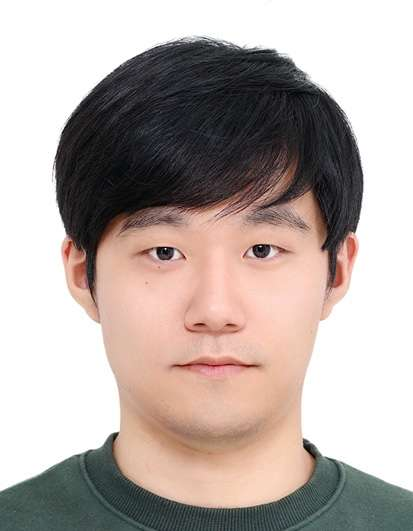
\includegraphics[width=.5\linewidth,height=.35\textheight]{moon.jpg}\\
		\textbf{문예찬 (Builder)}\\
		\textit{``창조의 손길''}\\
		\begin{flushleft}\footnotesize
			특징: 목 디스크, 허리디스크\\
			한마디: \textbf{적당한 알콜은 코딩을 도운다.}
		\end{flushleft}
	
		\column{0.48\textwidth}
		\centering
		
\includegraphics[width=.5\linewidth,height=.35\textheight]{kim.jpg}\\
		\textbf{김예찬 (Vaildator)}\\
		\textit{``오류 저격수''}\\
		\begin{flushleft}\footnotesize
			특징: 앱등이, 잠꾸러기\\
			한마디: \textbf{ 적당한 코딩은 알콜을 부른다.}
		\end{flushleft}
	\end{columns}
\end{frame}

\section{II. 전략은 우리의 무기!}
\begin{frame}{II.1 개발 목표}
	\begin{itemize}[<+->]
		\item 큰 정수에 대한 연산을 처리할 수 있는 라이브러리를 개발. \[
		a\pm b=?\quad a*b=?\quad a/b=?\quad a \bmod b=?\quad a^b\bmod{c}=?
		\]
		\item 라이브러리를 통한 BSGS 알고리즘으로 DLP 해독기 개발. \[
		g^x\equiv h\ (\bmod{n})\implies x=?
		\]
		% and so on
	\end{itemize}
\end{frame}
\begin{frame}{II.2 개발 전략}
	\begin{itemize}[<+->]
		\item 
		요구사항 분석: 지원될 작업 및 기능을 고려하여 라이브러리의 요구사항 및 사양을 정의합니다.
		\item 설계 및 구현: 다양한 정수 연산을 수행하기 위한 아키텍처를 설계하고 알고리즘을 구현합니다.
		\item 테스트 및 검증: 테스트 및 검증을 통해 라이브러리의 신뢰성과 정확성을 보장합니다.
	\end{itemize}
\end{frame}


\section{III. 라이브러리야, 너의 힘을 보여줘!}
\begin{frame}{IV.1 개발 라이브러리 소개 및 성능}
	% For a more dynamic slide, use overlays
	\begin{itemize}[<+->]
		\item Key Revenue Stream 1
		\item Key Revenue Stream 2
		% and so on
	\end{itemize}
\end{frame}

\section{IV. 라이브러리의 진가를 보여주지!}
\begin{frame}{라이브러리 활용}
	% For a more dynamic slide, use overlays
	\begin{itemize}[<+->]
		\item Key Revenue Stream 1
		\item Key Revenue Stream 2
		% and so on
	\end{itemize}
\end{frame}

\section{V. 역시 돈이 최고야!}
\begin{frame}{수익 모델}
	% For a more dynamic slide, use overlays
	\begin{itemize}[<+->]
		\item Key Revenue Stream 1
		\item Key Revenue Stream 2
		% and so on
	\end{itemize}
\end{frame}

\begin{frame}{Revenue Model}
	% For a more dynamic slide, use overlays
	\begin{itemize}[<+->]
		\item Key Revenue Stream 1
		\item Key Revenue Stream 2
		% and so on
	\end{itemize}
\end{frame}

\begin{frame}{Development Log}
	% Use tikz for custom graphics or flowcharts
	\begin{tikzpicture}
		% Custom tikz diagram here
	\end{tikzpicture}
\end{frame}

\begin{frame}{Conclusion}
	% Summarize the main points of your presentation
\end{frame}

\begin{frame}{Questions?}
	\centering \Large
	Any Questions?
\end{frame}

\end{document}